
\subsection{Cloud Service}\label{subsec:cloud-service}

\subsubsection{Architektur}

Es gibt deren Domänen 2. Configuration und Notification.

So quasi als ob man 2 Microservices haben kann. Aber wär halt doof das für den stand jetzt schon so zu trennen, deshalb vorerst mal erst ein einzelnes.

\clearpage

\subsubsection{Domänenmodell}


Für die beiden Domänen gibt es natürlich auch so n paar Diagramme. Die gibts jetzt hier:


\subsubsection*{Domäne Configuration}

\begin{figure}[h]
    \centering
    \begin{minipage}[b]{1.0\textwidth}
        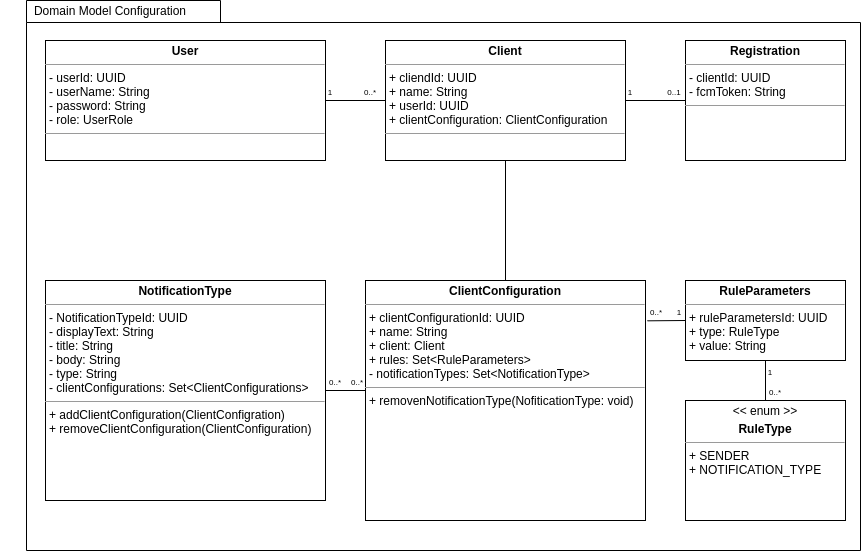
\includegraphics[width=\textwidth]{graphics/Class_Configuration_Domain}
        \caption{Domänenmodell Configuration}
    \end{minipage}
\end{figure}

\clearpage
\subsubsection*{Domäne Notification}

\begin{figure}[h]
    \centering
    \begin{minipage}[b]{1.0\textwidth}
        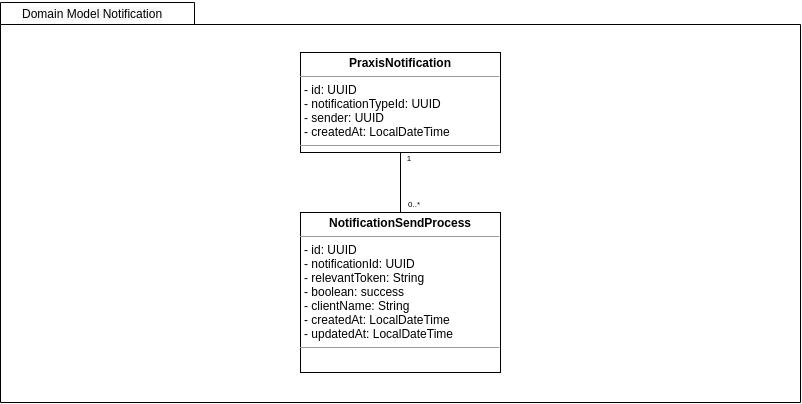
\includegraphics[width=\textwidth]{graphics/Class_Notification_Domain}
        \caption{Domänenmodell Notification}
    \end{minipage}
\end{figure}


\clearpage
\subsubsection{Laufzeitmodell}

\clearpage
